\documentclass[journal,12pt,twocolumn]{IEEEtran}

% Standard Packages
\usepackage{cite}
\usepackage{amsmath,amssymb,amsfonts,amsthm}
\usepackage{algorithmic}
\usepackage{graphicx}
\usepackage{textcomp}
\usepackage{xcolor}
\usepackage{listings}
\usepackage{enumitem}
\usepackage{mathtools}
\usepackage{gensymb}
\usepackage{comment}
\usepackage{tkz-euclide} 
\usepackage{gvv} 
\usepackage{longtable} 
\usepackage{calc} 
\usepackage{multirow}
\usepackage{hhline} 
\usepackage{tikz}
\usepackage{ifthen}
\usepackage{lscape}
\usepackage{tabularx}
\usepackage{float}

\renewcommand{\thetable}{\theenumi}
\theoremstyle{remark}

% Begin Document
\begin{document}

\bibliographystyle{IEEEtran}
\vspace{3cm}
\title{2011-ME-'40-52'}
\author{AI24BTECH11006 - Bugada Roopansha}
\maketitle

\begin{enumerate}[start=40]
 

    \item A spherical steel ball of $12$ mm diameter is initially at $1000$ K. It is slowly cooled in a surrounding of $300$ K. The heat transfer coefficient between the steel ball and the surrounding is $5 \frac{W}{m^2 K}$. The thermal conductivity of steel is $20 \frac{W}{mK}$. The temperature difference between the centre and the surface of the steel ball is
    \begin{enumerate}
        \item large because conduction resistance is far higher than the convective resistance.
        \item large because conduction resistance is far less than the convective resistance.
        \item small because conduction resistance is far higher than the convective resistance.
        \item small because conduction resistance is far less than the convective resistance.
    \end{enumerate}

    \item An ideal Brayton cycle, operating between the pressure limits of $1$ bar and $6$ bar, has minimum and maximum temperatures of $300$ K and $1500$ K. The ratio of specific heats of the working fluid is $1.4$. The approximate final temperatures in Kelvin at the end of the compression and expansion processes are respectively
    \begin{enumerate}
        \item $500$ and $900$
        \item $900$ and $500$
        \item $500$ and $500$
        \item $900$ and $900$
    \end{enumerate}

    \item A disc of mass $m$ is attached to a spring of stiffness $k$ as shown in the figure. The disc rolls without slipping on a horizontal surface. The natural frequency of vibration of the system is

    \begin{center}
    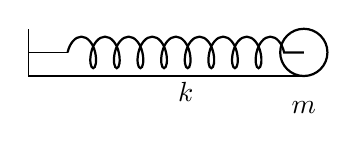
\begin{tikzpicture}
        % Drawing the spring
        \draw[thick, decoration={coil,aspect=0.5,segment length=3mm, amplitude=2mm}, decorate] (0,0) -- (3,0);
        \node at (1.5,-0.5) {$k$};

        % Drawing the disc
        \draw[thick] (3,0) circle (0.3);
        \node at (3,-0.7) {$m$};

        \draw (-0.5,-0.3) -- (3,-0.3);
        \draw (-0.5,0) -- (0,0);
        \draw (-0.5,-0.3) -- (-0.5,0.3);
    \end{tikzpicture}
    \end{center}


    \begin{enumerate}
        \item $\frac{1}{2\pi} \sqrt{\frac{k}{m}}$
        \item $\frac{1}{2\pi} \sqrt{\frac{2k}{m}}$
        \item $\frac{1}{2\pi} \sqrt{\frac{2k}{3m}}$
        \item $\frac{1}{2\pi} \sqrt{\frac{3k}{2m}}$
    \end{enumerate}


    \item A $1$ kg block is resting on a surface with coefficient of friction $\mu= 0.1$. A force of $0.8$ N is applied to the block as shown in the figure. The friction force is
    \begin{center}
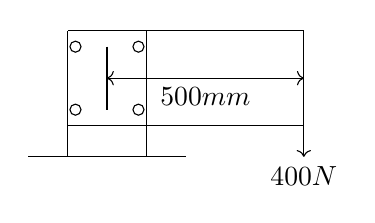
\begin{tikzpicture}
    % Draw rivets as circles
    \draw (0.4, 0.4) circle (2pt) node[above right] {};
    \draw (0.4, -0.4) circle (2pt) node[below right] {};
    \draw (-0.4, 0.4) circle (2pt) node[above left] {};
    \draw (-0.4, -0.4) circle (2pt) node[below left] {};

    

    % Draw horizontal and vertical distances between rivets
    \draw (0.5, 0.6) -- (-0.5, 0.6) ;
    \draw (0.5, -0.6) -- (-0.5, -0.6);
    \draw (-0.5, -0.6) -- (-0.5,0.6);
    \draw (0.5, -0.6) -- (0.5, 0.6);
    \draw (0.5, -0.6) -- (0.5, -1);
    \draw (-0.5, -0.6) -- (-0.5, -1);
   \draw (1, -1) -- (-1, -1);
    \draw (0.5, 0.6) -- (2.5, 0.6) ;
    \draw (0.5, -0.6) -- (2.5, -0.6) ;
    \draw (2.5 ,0.6) -- (2.5 ,-0.6);
    \draw[->] (2.5,-0.6) -- (2.5 ,-1) node[below]{$400N$} ;
    \draw (0,0.4) -- (0,-0.4);
    \draw[<->] (0,0) -- (2.5,0) node[below,midway]{$500 mm$};
\end{tikzpicture}
\end{center}

    \begin{enumerate}
        \item $0$
        \item $0.8$ N
        \item $0.98$ N
        \item $1.2$ N
    \end{enumerate}

    \item Consider the following system of equations:
    $$
    2x_1 + x_2 + x_3 = 0\\,
    x_2-x_3 = 0\\
 x_1 + x_2 = 0.
    $$
    This system has
    \begin{enumerate}
        \item a unique solution
        \item no solution
        \item an infinite number of solutions
        \item five solutions
    \end{enumerate}


    \item A single-point cutting tool with $12\degree$ rake angle is used to machine a steel workpiece. The depth of cut, i.e., uncut thickness is $0.81$ mm. The chip thickness under orthogonal machining conditions is $1.8$ mm. The shear angle is approximately
    \begin{enumerate}
        \item $22\degree$
        \item $26\degree$
        \item $56\degree$
        \item $76\degree$
    \end{enumerate}

    \item Match the following non-traditional machining processes with the corresponding material removal mechanisms:
    \begin{center}
        \begin{center}
    \begin{tabular}{|p{3cm}|p{3cm}|}
        \hline
        \textbf{Machining Process} & \textbf{Mechanism of Material Removal} \\
        \hline
        P. Chemical machining & $1.$ Erosion \\
        Q. Electro-chemical machining & $2.$ Corrosive reaction \\
        R. Electro-discharge machining & $3.$ Ion displacement \\
        S. Ultrasonic machining & $4.$ Fusion and vaporization \\
        \hline
    \end{tabular}
\end{center}


    \end{center}
    \begin{enumerate}
        \item P-$2$, Q-$3$, R-$4$, S-$1$
        \item P-$2$, Q-$4$, R-$3$, S-$1$
        \item P-$3$, Q-$2$, R-$4$, S-$1$
        \item P-$2$, Q-$3$, R-$1$, S-$4$
    \end{enumerate}

    \item A cubic casting of $50$ mm side undergoes volumetric solidification shrinkage and volumetric solid contraction of $4\%$ and $6\%$ respectively. No riser is used. Assume uniform cooling in all directions. The side of the cube after solidification and contraction is
    \begin{enumerate}
        \item $48.32$ mm
        \item $49.90$ mm
        \item $49.94$ mm
        \item $49.96$ mm
    \end{enumerate}



\textbf{Common Data for Questions 48 and 49:}\\ 
In an experimental set-up, air flows between two stations P and Q adiabatically. The direction of flow depends on the pressure and temperature conditions maintained at P and Q. The conditions at station P are $150$ kPa and $350$ K. The temperature at station Q is $300$ K. \\
The following are the properties and relations pertaining to air: \\
Specific heat at constant pressure, $c_p = 1.005 \frac{ kJ}{kgK}$; \\
Specific heat at constant volume, $c_v = 0.718\frac{ kJ}{kgK}$; \\
Characteristic gas constant, $R = 0.287 \frac{kJ}{kgK}$. \\
Enthalpy, $h = c_p T$. \\
Internal energy, $u = c_v T$. 


    \item If the air has to flow from station P to station Q, the maximum possible value of pressure in kPa at station Q is close to
    \begin{enumerate}
        \item $50$
        \item $87$
        \item $128$
        \item $150$
    \end{enumerate}

    \item If the pressure at station Q is $50$ kPa, the change in entropy $\brak{s_Q - s_P}$ in $\frac{kJ}{kgK}$ is
    \begin{enumerate}
        \item $-0.155$
        \item $0$
        \item $0.160$
        \item $0.355$
    \end{enumerate}

\textbf{Common Data for Questions 50 and 51:} \\
One unit of product $P_1$ requires $3$ kg of resource $R_1$, and $1$ kg of resource $R_2$. One unit of product $P_2$ requires $2$ kg of resource $R_1$, and $2$ kg of resource $R_2$. The profits per unit by selling product $P_1$ and $P_2$ are Rs. $2000$ and Rs. $3000$ respectively. The manufacturer has $90$ kg of resource $R_1$ and $100$ kg of resource $R_2$.

    \item The unit worth of resource $R_2$, i.e., the dual price of resource $R_2$ in Rs. per kg is
    \begin{enumerate}
        \item $0$
        \item $1350$
        \item $1500$
        \item $2000$
    \end{enumerate}

    \item The manufacturer can make a maximum profit of Rs.
    \begin{enumerate}
        \item $60000$
        \item $135000$
        \item $150000$
        \item $200000$
    \end{enumerate}



\textbf{Statement for Linked Answer Questions 52 and 53:} \\
A triangular-shaped cantilever beam of uniform thickness is shown in the figure. The Young's modulus of the material of the beam is $E$. A concentrated load $P$ is applied at the free end of the beam.


    \item The area moment of inertia about the neutral axis of a cross-section at a distance $x$ measured from the free end is
    \begin{enumerate}
        \item $\frac{b x t^3}{6l}$
        \item $\frac{b x t^3}{12l}$
        \item $\frac{b x t^3}{24l}$
        \item $\frac{ x t^3}{12}$
    \end{enumerate}

    

    




    


\end{enumerate}

\end{document}

